%%%%%%%%%%%%%%%%%%%%%%%%%%%%%%%%%%%%%%%%%
% University/School Laboratory Report
% LaTeX Template
% Version 3.1 (25/3/14)
%
% This template has been downloaded from:
% http://www.LaTeXTemplates.com
%
% Original author:
% Linux and Unix Users Group at Virginia Tech Wiki 
% (https://vtluug.org/wiki/Example_LaTeX_chem_lab_report)
%
% License:
% CC BY-NC-SA 3.0 (http://creativecommons.org/licenses/by-nc-sa/3.0/)
%
%%%%%%%%%%%%%%%%%%%%%%%%%%%%%%%%%%%%%%%%%

%----------------------------------------------------------------------------------------
%	PACKAGES AND DOCUMENT CONFIGURATIONS
%----------------------------------------------------------------------------------------

\documentclass{article}

\usepackage[version=3]{mhchem} % Package for chemical equation typesetting
\usepackage{siunitx} % Provides the \SI{}{} and \si{} command for typesetting SI units
\usepackage{graphicx} % Required for the inclusion of images
\usepackage{natbib} % Required to change bibliography style to APA
\usepackage{amsmath} % Required for some math elements 
\usepackage[utf8]{inputenc}
\usepackage{tikz,pgfplots}
\usepackage[letterpaper, margin=0.2in]{geometry}
\usepackage{float}
\usepackage{enumitem}
\usepackage{fixltx2e}
\usepackage{gensymb}
\usepackage[hidelinks]{hyperref}
\usepackage[all]{hypcap}

\usepackage{xcolor}

% Roman numerials
\pagenumbering{arabic}

\setlength\parindent{0pt} % Removes all indentation from paragraphs

%\renewcommand{\labelenumi}{\alph{enumi}.} % Make numbering in the enumerate environment by letter rather than number (e.g. section 6)

%\usepackage{times} % Uncomment to use the Times New Roman font

% for some tables
\newcommand{\specialcell}[2][c]{%
  \begin{tabular}[#1]{@{}c@{}}#2\end{tabular}}
  
\providecommand{\e}[1]{\ensuremath{\times 10^{#1}}}
%----------------------------------------------------------------------------------------
%	DOCUMENT INFORMATION
%----------------------------------------------------------------------------------------

%\title{Determination of the Atomic \\ Weight of Magnesium \\ CHEM 101} % Title

%\author{John \textsc{Smith}} % Author name

%\date{\today} % Date for the report

\begin{document}

%\maketitle % Insert the title, author and date

% If you wish to include an abstract, uncomment the lines below
% \begin{abstract}
% Abstract text
% \end{abstract}

%----------------------------------------------------------------------------------------
%	SECTION 1
%----------------------------------------------------------------------------------------


\section{SVD Analysis}
\subsection{noise reduction}

\Large{SVDs can be used in a number of ways to improve TBT BPM data. One example would be reducing the noise in individual BPMs. This can be done by computing an SVD then setting all singular values due to noise to zero and recomputing the BPM matrix. This method reduces the noise by a factor of $\sqrt{\frac{d}{M}}$ where d is the dimension of signal space (\# of singular values that were not zeroed) and M is the \# of BPMs. \\*[1cm]

\large{\textbf{example 1:}} Simulated 10,000 turns starting with a 3mm kick in both transverse planes. Additionally a gaussian noise distribution was added to the data with a mean of 0 and std $\sigma = 0.5$ mm. The graph below shows the ability of an SVD to be able to recover the noise that was manually added.

\begin{figure}[H]
\centering
\begin{tikzpicture}
\node at (0,0) {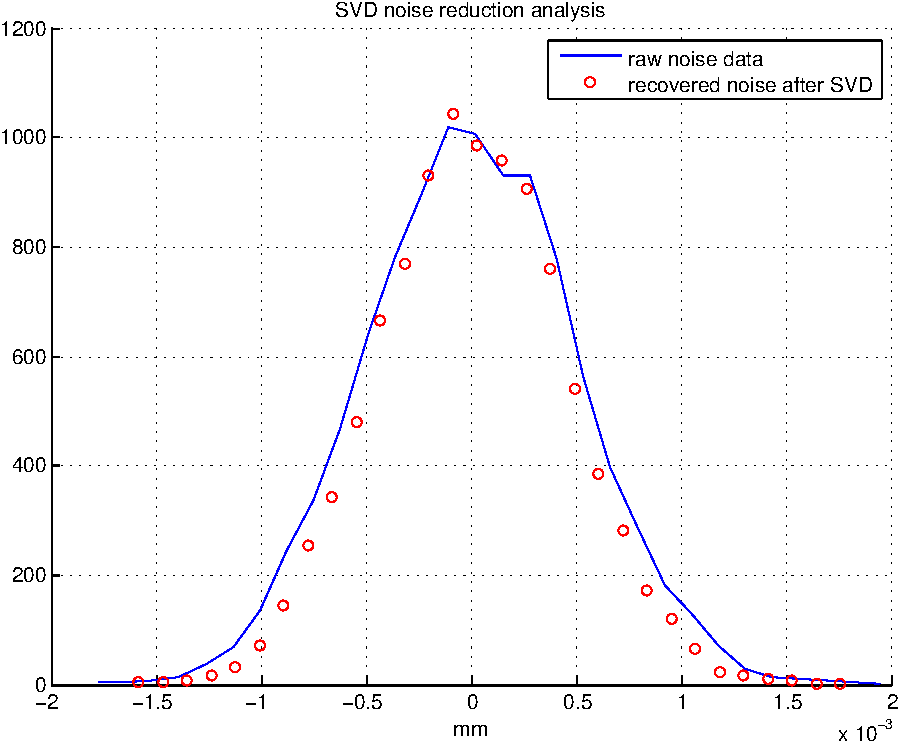
\includegraphics[width=400pt]{bpm_noise_reduction1.pdf}};
\end{tikzpicture}
\caption{}
\end{figure}

\textcolor{white}{l} \\*[4cm]

\large{\textbf{example 2:}} Using the same technique with data taken during beam excitation (using a pinger magnet) we can see that the noise reduction works equally as well. Looking at the FFT spectrum, we see that the tune amplitude was slightly improved while everything else (noise) was reduced.

\begin{figure}[H]
\centering
\begin{tikzpicture}
\node at (0,0) {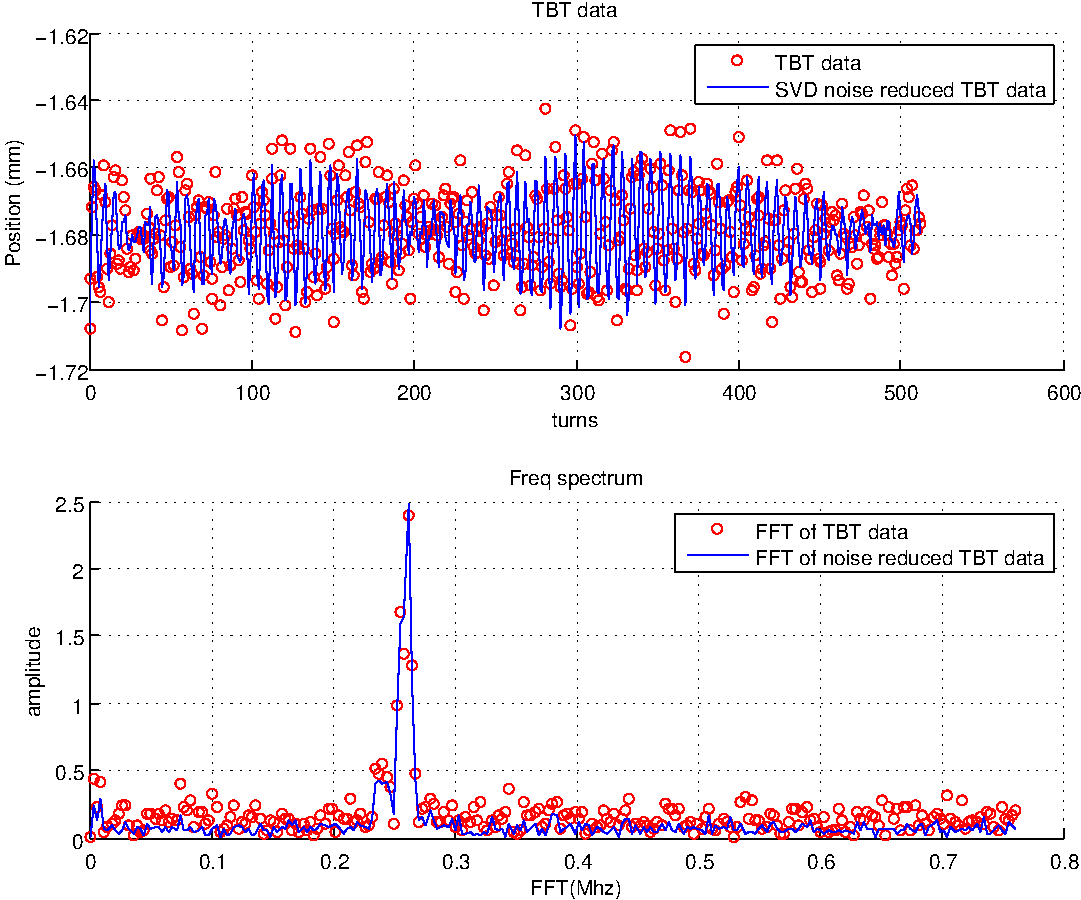
\includegraphics[width=400pt]{bpm_noise_reduction_pinger1.pdf}};
\draw[->] (-2.7,-0.5) -- (-1.8,-0.75);
\node at (-4,-0.5) {increased peak};
\end{tikzpicture}
\caption{}
\end{figure}

%\textcolor{white}{l} \\*[2cm]

\subsection{degrees of freedom with singular values}

By further looking into the singular values generated by an SVD we are able to pinpoint noisy BPMs. To do this we run an SVD with an increasing number of BPMs and plot there corresponding singular values. i.e. run an SVD with 1 BPM, grab top few singular values then repeat with 2 BPMs, then with 3 BPMs etc... \\*[1cm]

\large{\textbf{example 3:}} Using the same simulated data above, we create a degrees of freedom plot using the top 5 singular values. Note that flat lines correspond to noise in the singular values while a growing line indicates coherent beam signal. The step functions tell us about individual noisy/problematic BPMs in the data. The largest singular value (blue line) is due to the betatron mode (usually there should be two singular values corresponding to the two betatron modes).

\begin{figure}[H]
\centering
\begin{tikzpicture}
\node at (0,0) {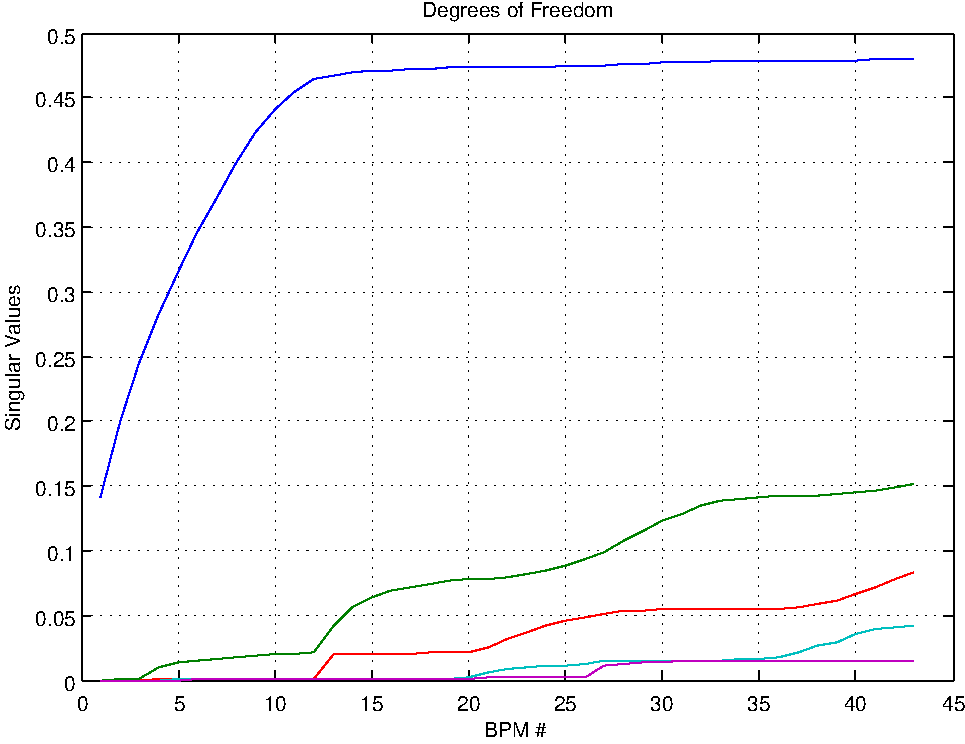
\includegraphics[width=400pt]{bpm_degrees_plot_sim1.pdf}};
\node at (2,1.2) {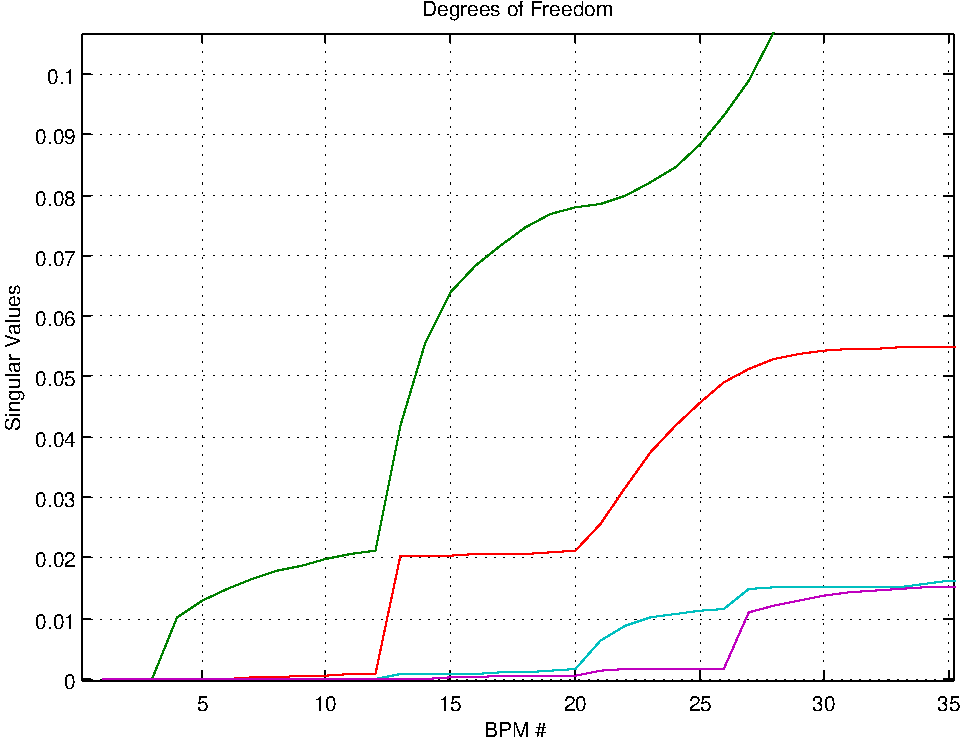
\includegraphics[width=240pt]{bpm_degrees_plot_simZoom1.pdf}};
\draw (-5.8,-4.65) -- (4.0,-4.65) -- (4.0,-2.5) -- (-5.8,-2.5) -- (-5.8,-4.65);
\draw (-5.8,-2.5) -- (-1.5,4.2);
\draw (4.0,-2.5) -- (6.1,-1.5);
\end{tikzpicture}
\caption{Note our noisy BPM (\# 27) has a step function. However another BPM (\# 13) seems to also have a step function which is weird as no artificial noise was added to any BPM except \# 27.}
\end{figure}

\subsection{spatial and temporal vectors}

By looking at the spatial and temporal vectors generated by an SVD, we can further pinpoint individual noisy/bad BPMs. \\*[1cm]

\large{\textbf{example 3:}} Looking at the same simulated data from example 1, we can detect which BPM the gaussian noise was added to very easily. Going through each spatial vector corresponding to each singular value, we are able to find our noisy BPM (BPM \# 27).

\begin{figure}[H]
\centering
\begin{tikzpicture}
\node at (0,0) {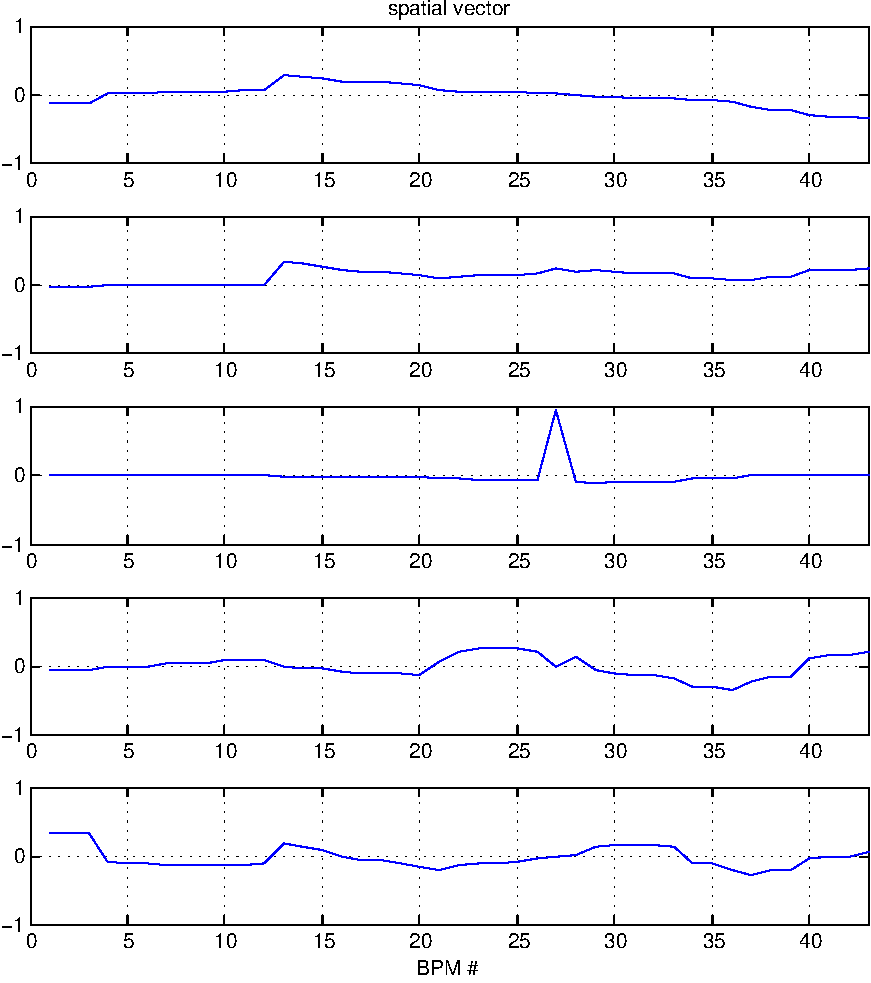
\includegraphics[width=400pt]{bpm_spatial_noise_bpm271.pdf}};
\end{tikzpicture}
\caption{By cycling through a few spatial vectors we can easily see that in the middle graph there is a huge spike at BPM \# 27, which is our gaussian noise induced BPM.}
\end{figure}


%	SECTION 5
%----------------------------------------------------------------------------------------


%----------------------------------------------------------------------------------------
%	SECTION 6
%----------------------------------------------------------------------------------------

% Nothing right now

%----------------------------------------------------------------------------------------
%	BIBLIOGRAPHY
%----------------------------------------------------------------------------------------

\bibliographystyle{apalike}

\bibliography{sample}

%----------------------------------------------------------------------------------------


\end{document}













